\chapter{Results}
\label{chap:results}

This chapter begins with a description of the experimental setup and key assumptions. We then give a brief overview of the dataset. The main section evaluates and compares different versions of our model, focusing on how each added component affects performance. Finally, we explore how the model's performance depends on the number of training experiments.

To simplify notation throughout this chapter, we use the following abbreviations for the model layers: X\_ON and X\_OFF represent the LGN ON and OFF cell populations. V1\_Exc\_L4 and V1\_Inh\_L4 refer to the excitatory and inhibitory cell populations in V1 layer 4, and V1\_Exc\_L23 and V1\_Inh\_L23 refer to those in V1 layer 2/3. These match the layer names used in our model code and will be used consistently throughout.

\section{Experimental Setup and Technicalities}
\label{sec:experimental_setup}

Unless otherwise specified, all experiments were run using the model setup and artificial dataset described in Chapter~\ref{chap:methods}.

In addition to the setup from the previous chapter, we used several parameters chosen based on our experience during model development. These were mostly influenced by practical constraints such as limited GPU access, memory availability, or model-specific issues. Because thorough testing of all parameter combinations would have required too many resources, we selected values that we believed were reasonable. While we do not expect these parameters to drastically affect our findings, they could be optimized in future work.

ne important parameter is the batch size. As explained in Section~\ref{sec:artificial_dataset}, our dataset is made up of samples that each represent a single experiment. These had to be grouped into batches for training. We chose a batch size of $50$ based on a balance of performance and hardware limits. Training RNNs on time-based data is typically slow, since computations must happen in sequence and cannot be easily parallelized. Using larger batch sizes allows some parallel processing on GPUs, which helps speed things up. However, larger batches also require more memory.

Memory demands were particularly high when using certain RNN neuronal modules, described in Section~\ref{subsec:additional_modules}, that rely on truncated backpropagation through time (TBPTT). TBPTT increases memory use significantly, especially when paired with small shared neural networks used in place of typical activation functions. To reduce this load, we merged time bins into 20~ms intervals, as described in Section~\ref{subsubsec:time_bins_merging}, which helped but did not fully solve the issue. As noted in Section~\ref{subsubsec:subset_selection}, we also had to limit our model to just 10\% of the artificial neurons from each layer of the original SNN template to stay within memory limits. After weighing all these factors, we chose a batch size of $50$, which worked reliably even with the most memory-intensive versions of our model, like the one using the synaptic depression module (Section~\ref{subsubsec:synaptic_depression}).

Another training safeguard we used was gradient clipping, which prevents gradients from growing too large and causing numerical issues. In all our experiments, we clipped gradients to a maximum value of 10,000. This was mainly a precaution to avoid overflow errors during training, especially during early development phases when we were experimenting with activation functions other than LeakyTanh. This topic is discussed further in Section~\ref{subsubsec:leakytanh}. In our final models, this gradient clipping had little to no effect on performance, but we kept it in place to ensure stability.

Finally, we want to mention the hardware used to run our experiments. Most were carried out on the Metacentrum computing cluster. While not every model variant needed a large GPU, we generally used GPUs with at least 40~GB of RAM. These are well-suited for deep learning tasks and were essential for models that relied on TBPTT. We also used machines with at least 8 CPU cores and 100~GB of RAM to support the computational load.


\section{Dataset Overview}
\label{sec:dataset_overview}

In this section, we present a statistical analysis of our dataset and evaluate the impact of the dataset simplifications we applied. First, we assess the effect of merging time bins from 1~ms to 20~ms, followed by an analysis of the influence of selecting a random subset comprising 10\% of neurons. All scripts used for this analysis are provided in the supplementary materials and the project's GitHub repository.

\subsection{Time Bin Merging Analysis}
\label{subsec:time_bin_merging_analysis}
As described in Section~\ref{subsubsec:time_bins_merging}, we merged the original 1~ms time bins into 20~ms intervals to accelerate computation and reduce data noisiness, while maintaining sufficient temporal resolution. We performed experiments using five bin sizes: 1~ms, 5~ms, 10~ms, 15~ms, and 20~ms. Due to the high computational cost of reprocessing the dataset for each binning size, we limited the analysis to this subset. Each configuration required substantial memory for processing and storage, which constrained the number of variants we could feasibly evaluate. The binning was introduced to significantly accelerate model training and reduce memory consumption.

\subsubsection{Total Spike Counts Across Time Bins}
\label{subsubsec:spike_counts_time_bins}

We begin by comparing the distribution of spike counts across all time bins for each binning size. We hypothesize the following:

\begin{claim}[Distribution of Spike Counts Across All Time Bins]
    The distribution of spike counts across time bins remains similar for bin sizes \{1, 5, 10, 15, 20\}~ms. This suggests that the temporal behavior of neuronal responses is largely preserved.
\end{claim}
\label{claim:tim_bin_counts}

Our assumption is that maintaining the binary-like properties of spike data should also preserve its temporal characteristics. Tables~\ref{tab:train_bin_count_distribution} and~\ref{tab:test_bin_count_distribution} show spike count distributions for the training and test datasets, respectively.

\begin{table}
    \centering\footnotesize\sf
    \begin{tabular}{cccccc}
    \toprule
        Spike Count & 1 ms & 5 ms & 10 ms & 15 ms & 20 ms \\
        \midrule
        0 & 0.9944 & 0.9727 & 0.9491 & 0.9287 & 0.9105 \\
        1 & 0.0056 & 0.0266 & 0.0460 & 0.0598 & 0.0710 \\
        2 & 0.0000 & 0.0007 & 0.0046 & 0.0100 & 0.0147 \\
        3 & 0.0000 & 0.0000 & 0.0003 & 0.0013 & 0.0032 \\
        4 & 0.0000 & 0.0000 & 0.0000 & 0.0001 & 0.0005 \\
        5 & 0.0000 & 0.0000 & 0.0000 & 0.0000 & 0.0001 \\
    \addlinespace % a nice non-intrusive separator of data groups (or final table sums)
    \bottomrule
    \end{tabular}
    \caption{\textbf{Spike count distribution in the train dataset:} This table shows the proportion of time bins containing 0 to 5 spikes for different time bin sizes. Spike counts above 5 are omitted as they occur rarely and have a negligible impact on the overall distribution.}
    \label{tab:train_bin_count_distribution}
\end{table}
    

\begin{table}
    \centering\footnotesize\sf
    \begin{tabular}{cccccc}
    \toprule
        Spike Count & 1 ms & 5 ms & 10 ms & 15 ms & 20 ms \\
    \midrule
        0 & 0.9944 & 0.9728 & 0.9493 & 0.9290 & 0.9107 \\
        1 & 0.0056 & 0.0265 & 0.0458 & 0.0597 & 0.0710 \\
        2 & 0.0000 & 0.0007 & 0.0045 & 0.0099 & 0.0146 \\
        3 & 0.0000 & 0.0000 & 0.0003 & 0.0013 & 0.0032 \\
        4 & 0.0000 & 0.0000 & 0.0000 & 0.0001 & 0.0005 \\
        5 & 0.0000 & 0.0000 & 0.0000 & 0.0000 & 0.0001 \\
    \addlinespace % a nice non-intrusive separator of data groups (or final table sums)
    \bottomrule
    \end{tabular}
    \caption{\textbf{Spike count distribution in the test dataset:} This table shows the proportion of time bins containing 0 to 5 spikes for different time bin sizes. Spike counts above 5 are omitted as they occur rarely and have a negligible impact on the overall distribution.}
    \label{tab:test_bin_count_distribution}
\end{table}

The distributions for both training and test sets are highly similar. Most time bins contain either zero or one spike, and only a small proportion include more than one. For the 20~ms bins, about 1.5\% of time bins contain two or more spikes. Notably, the percentage of time bins with at least one spike increases from roughly 0.6\% (1~ms bins) to 7\% (20~ms bins). This reduction in sparsity supports the hypothesis that the 20~ms bin size offers a reasonable balance between temporal resolution and data density.

Figures~\ref{fig:spike_count_distribution_train} and~\ref{fig:spike_count_distribution_test} further illustrate this by showing spike count distributions across all neuronal populations.

\begin{figure}
    \centering
    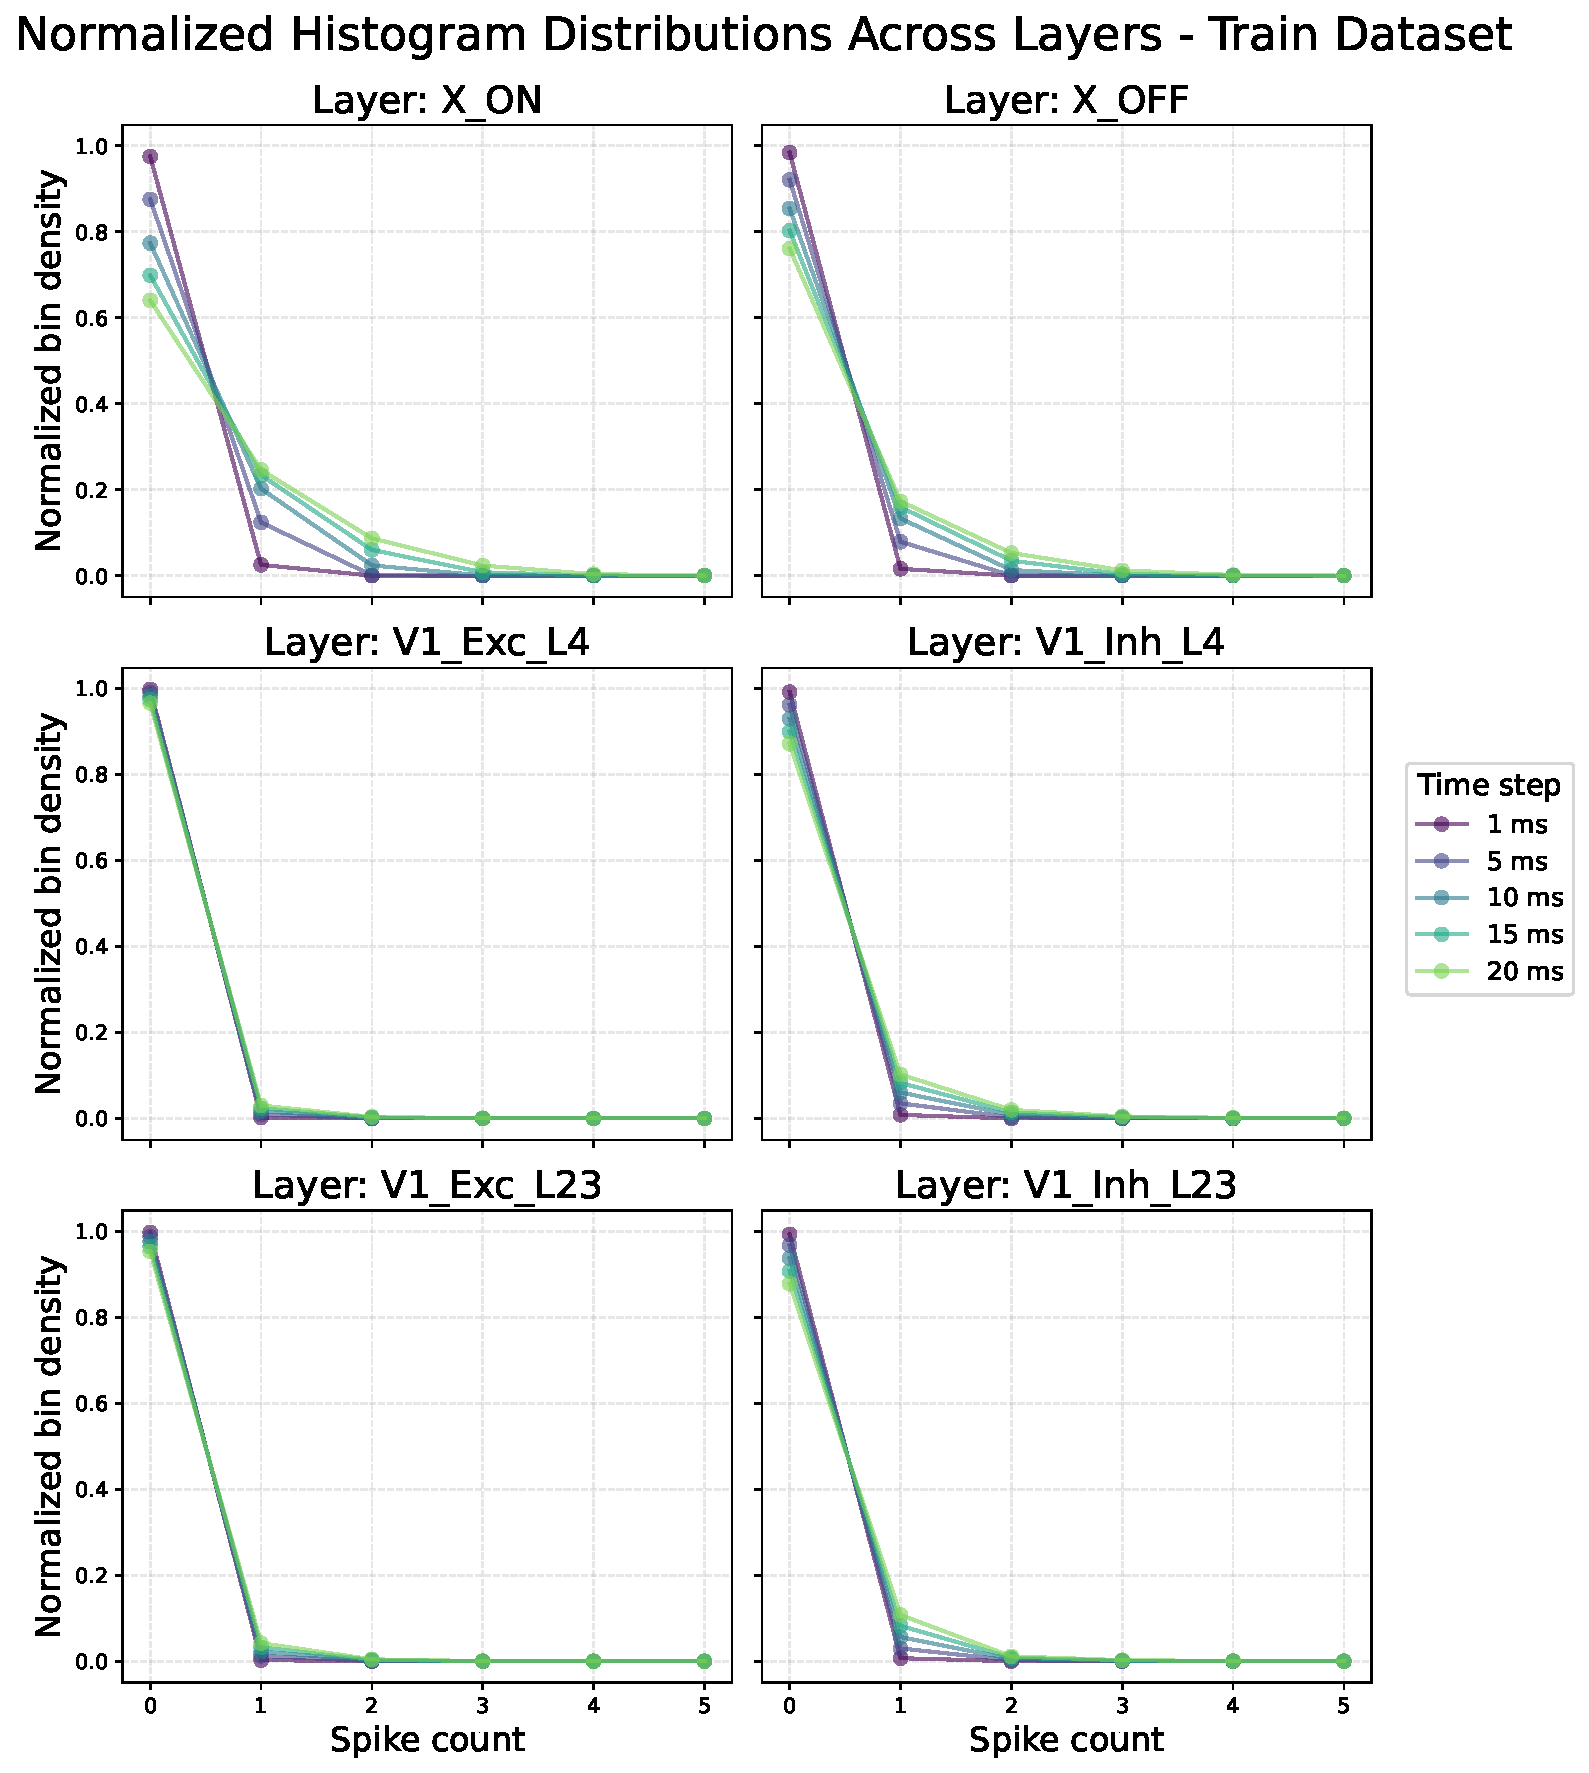
\includegraphics[width=\linewidth]{img/plots/time_step_counts_train.pdf}
    \caption{Evolution of spike counts per time bin with increasing bin size across all neuronal populations in the train dataset.}
    \label{fig:spike_count_distribution_train}
\end{figure}

\begin{figure}
    \centering
    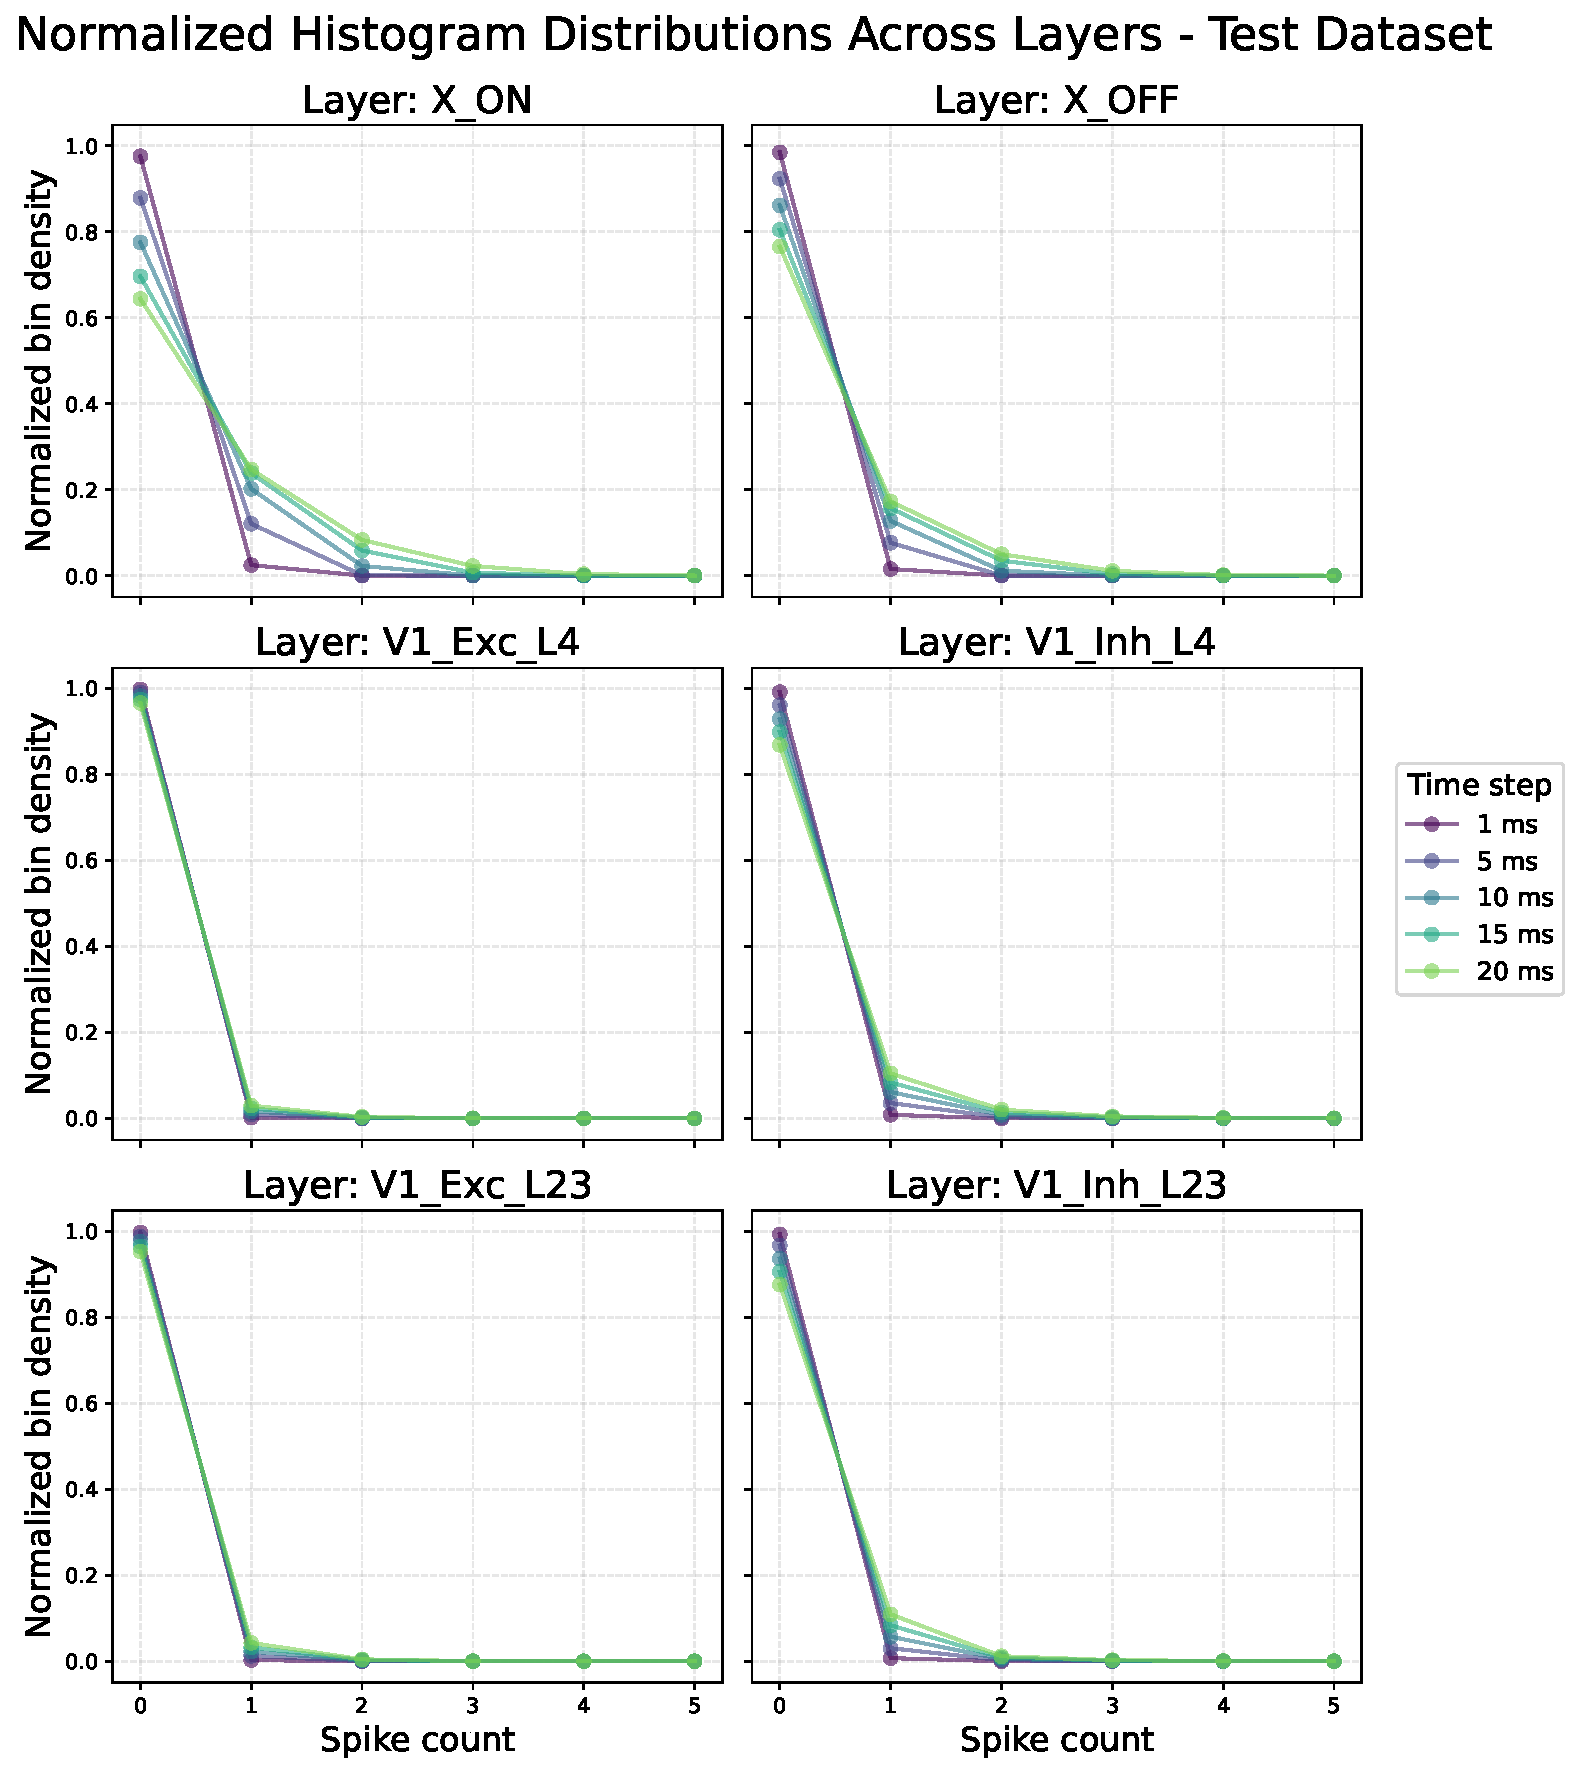
\includegraphics[width=\linewidth]{img/plots/time_step_counts_test.pdf}
    \caption{Evolution of spike counts per time bin with increasing bin size across all neuronal populations in the test dataset.}
    \label{fig:spike_count_distribution_test}
\end{figure}


\subsubsection{Spike Count Distribution Across Time}
\label{subsubsec:spike_time_distribution}
Next, we examine the distribution of spike counts across time for different bin sizes. We propose the following:

\begin{claim}[Temporal Spike Count Distribution]
    The temporal distribution of spike counts per experiment remains consistent across all tested bin sizes. This supports the preservation of temporal response patterns.
\end{claim}

Figures~\ref{fig:temporal_spike_distribution_train} and~\ref{fig:temporal_spike_distribution_test} show the mean spike counts over time for all neuronal populations in the training and test datasets, respectively. These distributions were interpolated to the 1~ms time scale using cubic interpolation.

\begin{figure}
    \centering
    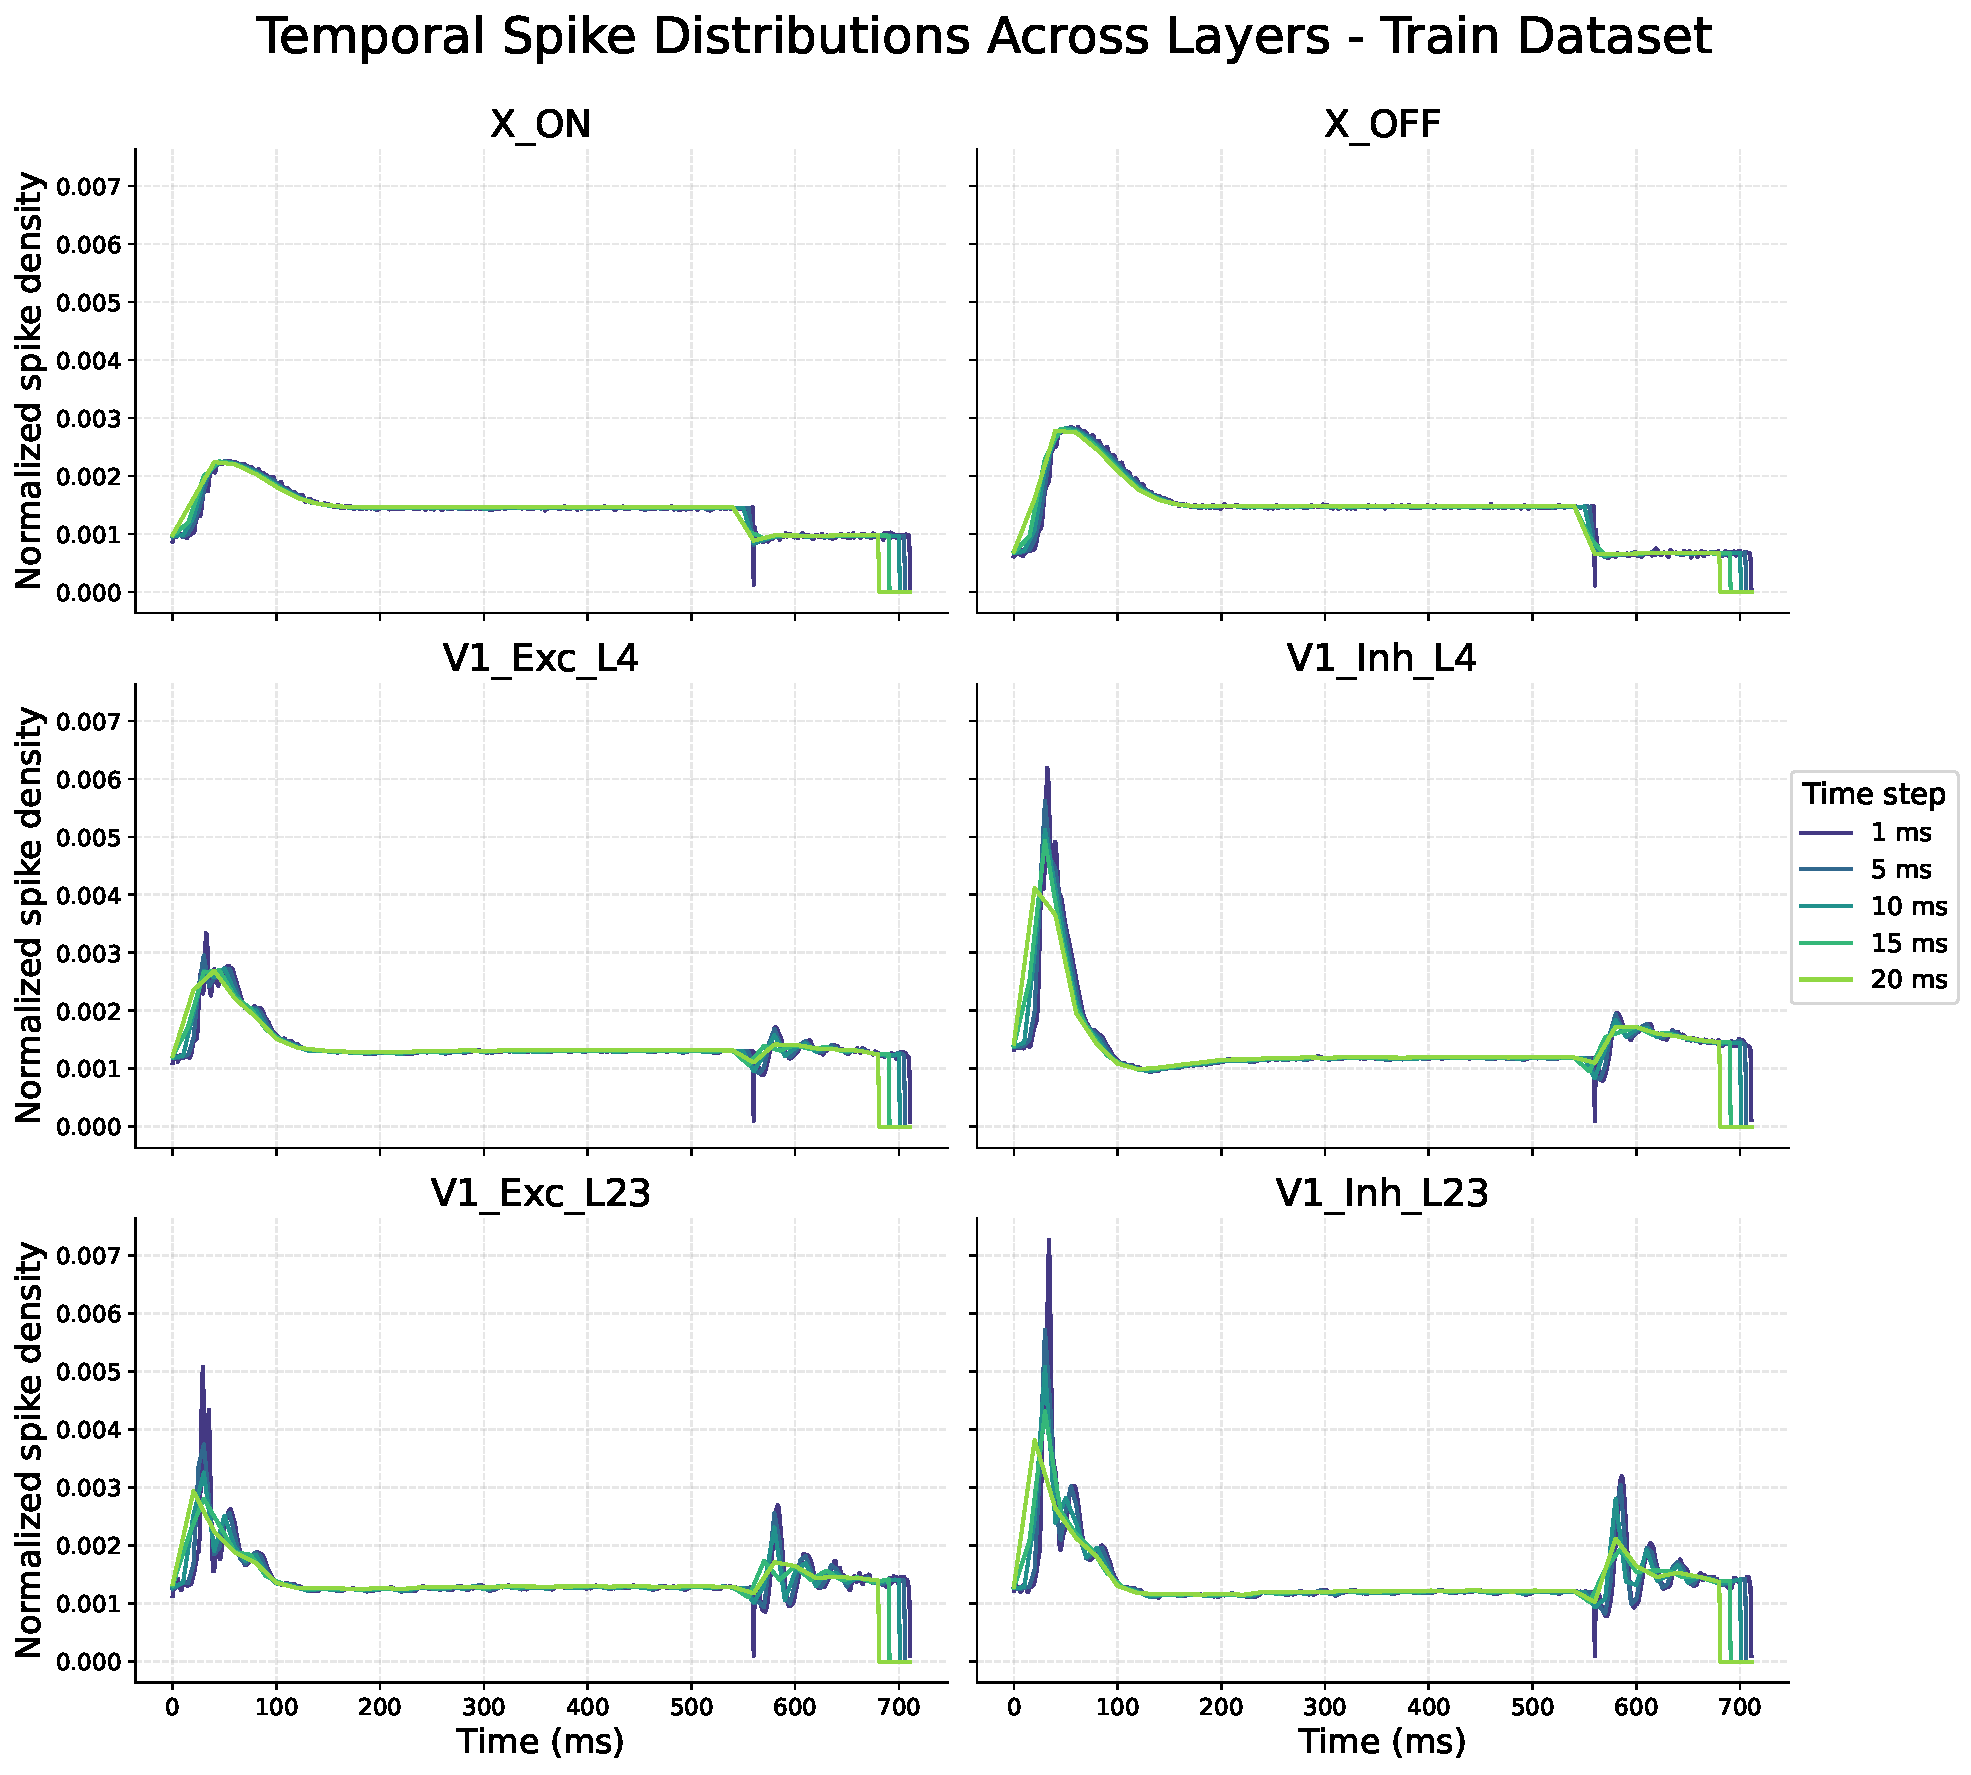
\includegraphics[width=\linewidth]{img/plots/temporal_spike_distribution_train.pdf}
    \caption{Comparison of temporal spike count distributions for different time bin sizes across all neuronal populations in the train dataset. The curves are interpolated to the original 1~ms resolution using cubic interpolation to improve line smoothness.}
    \label{fig:temporal_spike_distribution_train}
\end{figure}

\begin{figure}
    \centering
    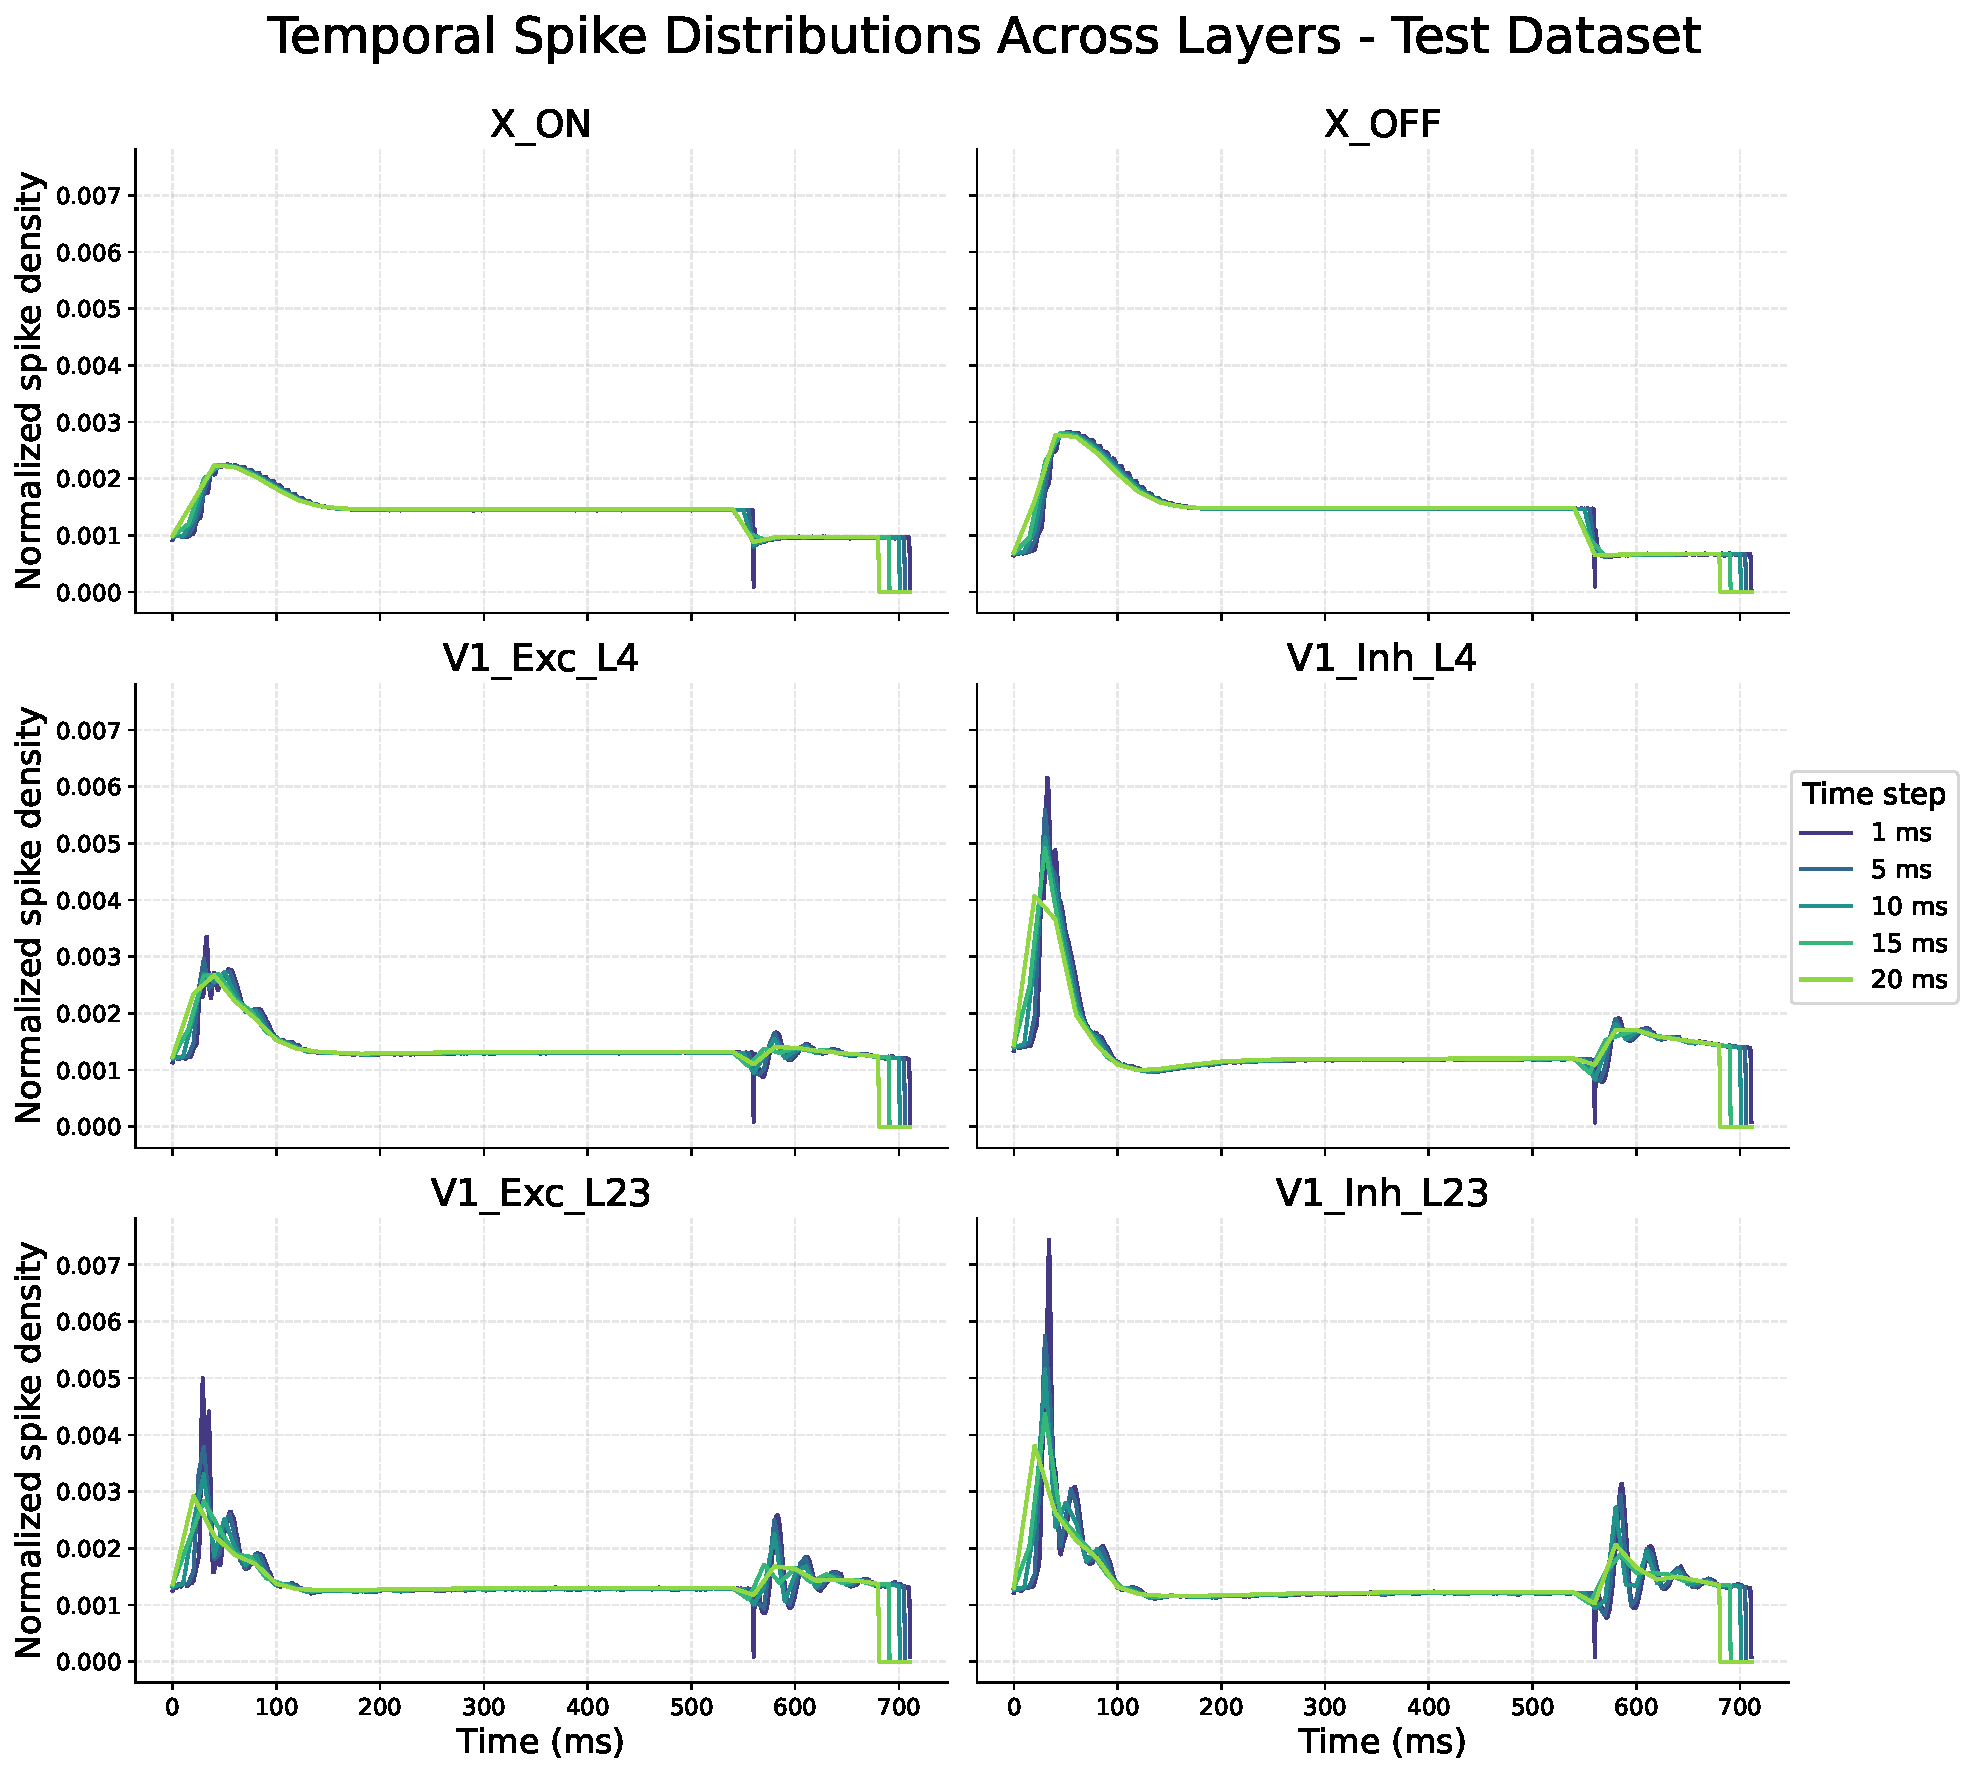
\includegraphics[width=\linewidth]{img/plots/temporal_spike_distribution_test.pdf}
    \caption{Comparison of temporal spike count distributions for different time bin sizes across all neuronal populations in the test dataset. The curves are interpolated to the original 1~ms resolution using cubic interpolation to improve line smoothness.}
    \label{fig:temporal_spike_distribution_test}
\end{figure}

These plots show a clear reduction in noise with increasing bin size, particularly in excitatory layers. The training dataset appears noisier than the test set, likely due to the test set's smaller size and the averaging effect of multiple trials per experiment.

Importantly, the overall distribution shape is preserved across bin sizes. This indicates that binning effectively reduces noise without substantially altering temporal dynamics. Heatmaps in Figure~\ref{fig:correlation_time_bin_size} display Pearson correlation coefficients across different bin sizes, confirming strong similarity in spike distributions over time.

\begin{figure}
    \centering
    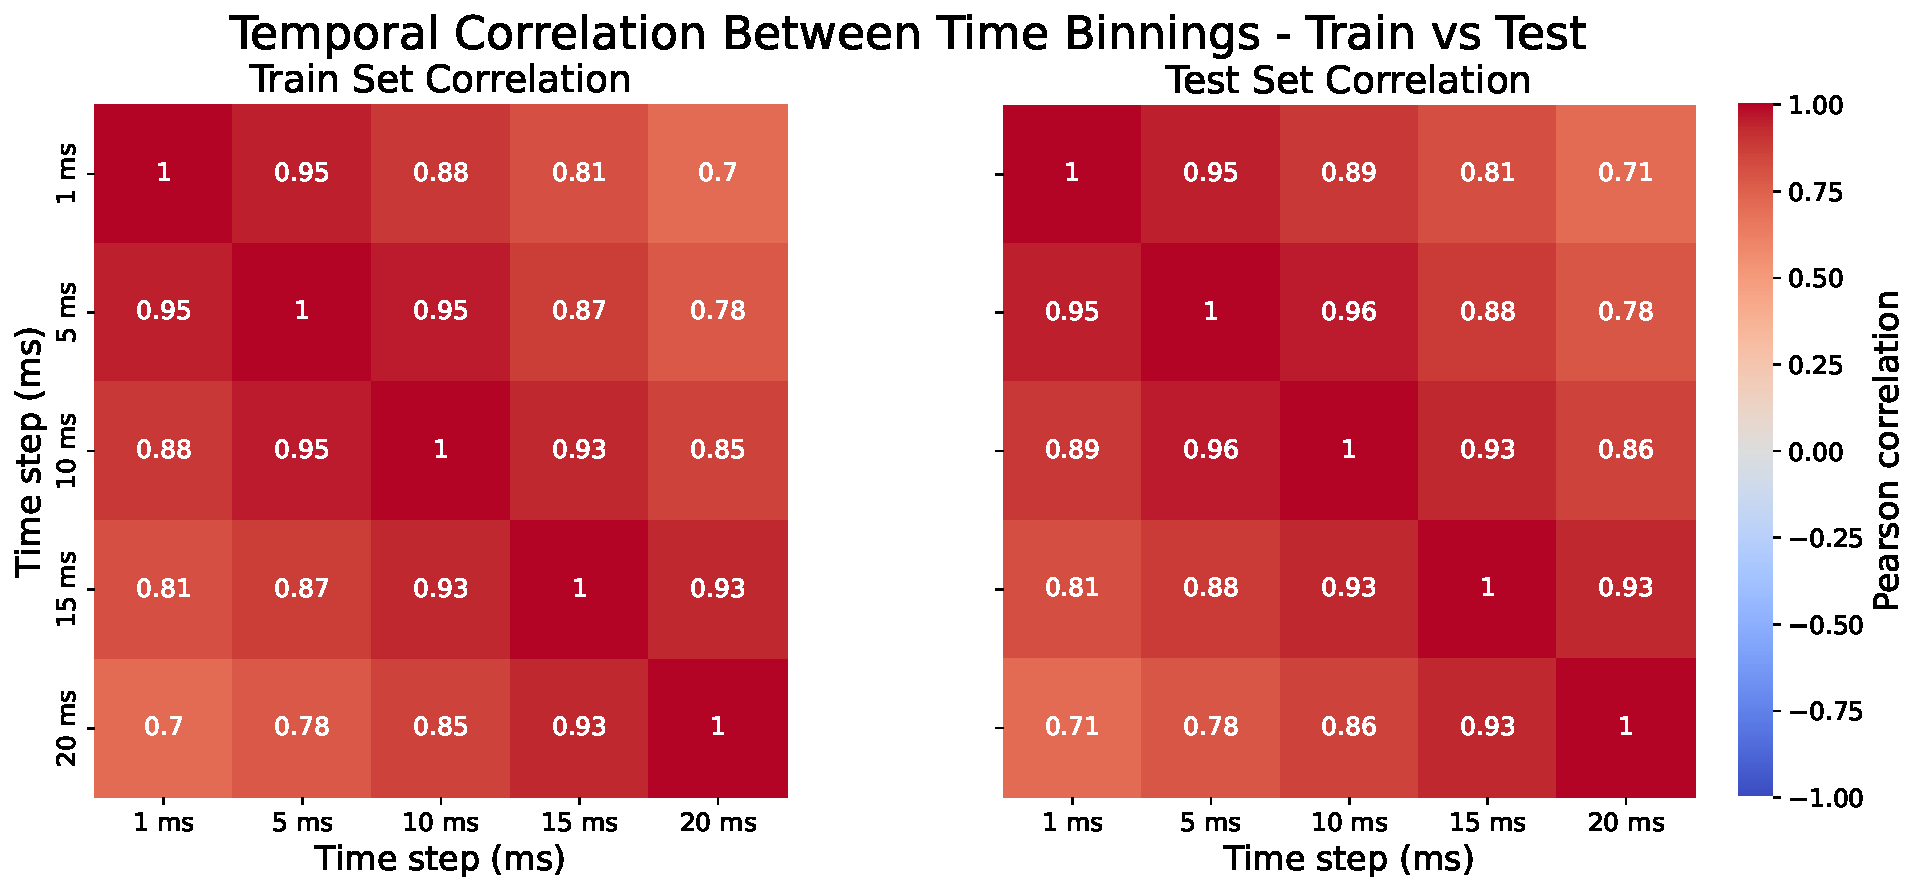
\includegraphics[width=\linewidth]{img/plots/temporal_correlation_time_bin_size.pdf}
    \caption{Heatmaps of Pearson correlation coefficients for spike count distributions over time between different time bin sizes in the train and test datasets.}
    \label{fig:correlation_time_bin_size}
\end{figure}

\subsubsection{Synchrony of Neuronal Populations in Different Time Bins}
\label{subsubsec:neuron_synchrony_binning}

Lastly, we evaluate how time binning affects synchrony, the proportion of neurons firing simultaneously within the same time bin. Synchrony provides insight into the collective temporal dynamics of neuronal populations and is widely studied in neuroscience (\citet{Singer1999}).

Our analysis focuses on the mean synchrony across all time steps. We state the following:

\begin{claim}[Synchrony of Neuronal Populations Across Time Bins]
    The mean synchrony of neuronal populations remains consistent across different time bin sizes. This implies that temporal structure of the dataset is largely preserved.
\end{claim}
\label{claim:synchrony_time_bins_size}

Figures~\ref{fig:boxplot_synchrony_time_train} and~\ref{fig:boxplot_synchrony_time_test} show synchrony distributions for each layer in the training and test datasets. Tables~\ref{tab:synchrony_time_bins_summary_train} and~\ref{tab:synchrony_time_bins_summary_test} summarize the mean and variance of synchrony values.

\begin{figure}
    \centering
    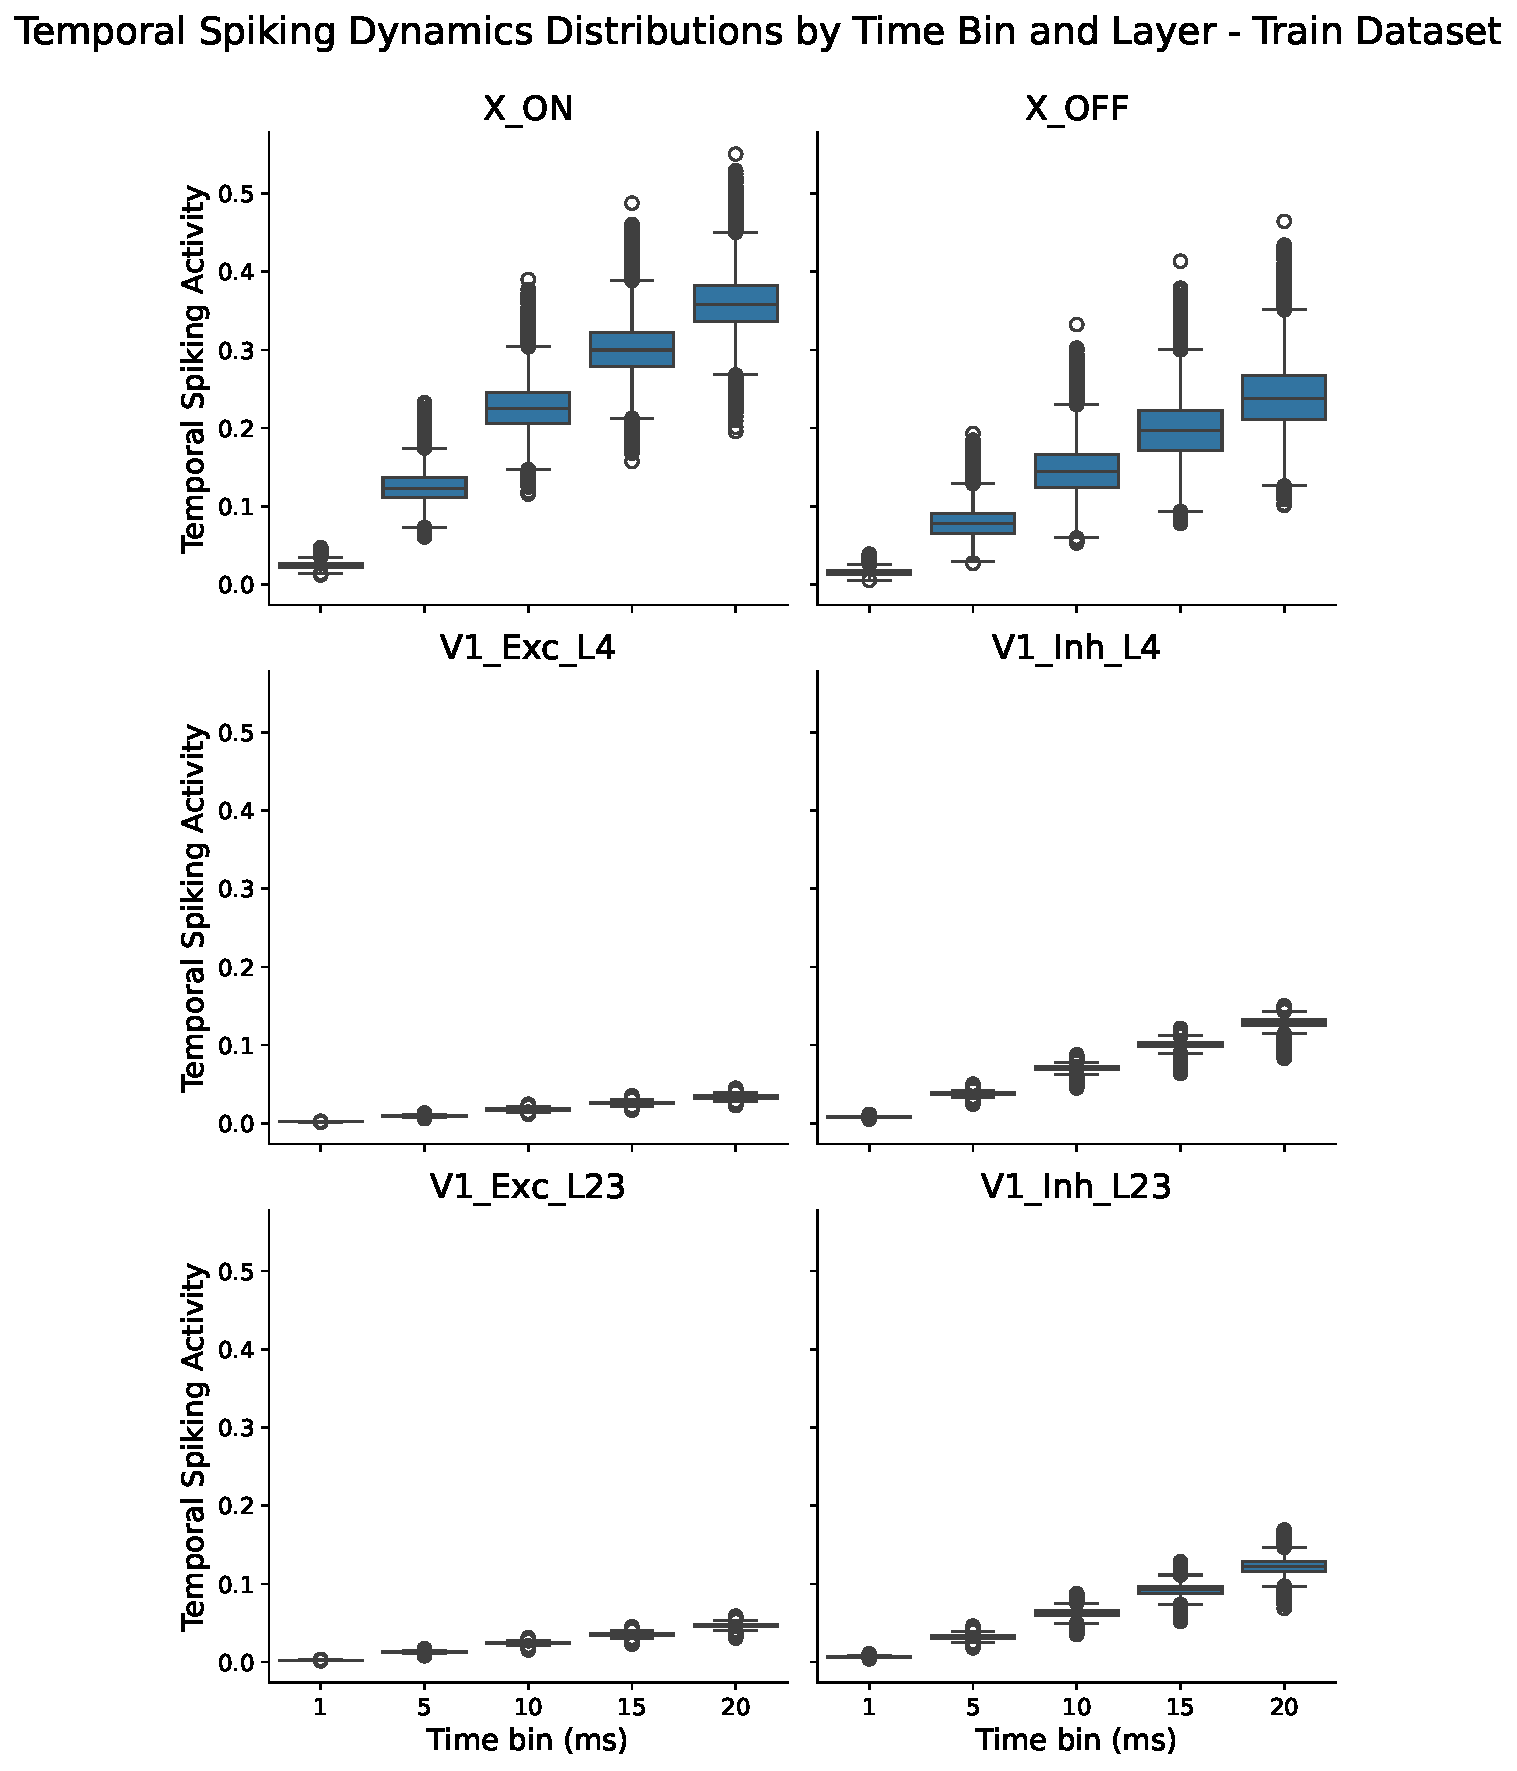
\includegraphics[width=0.92\linewidth]{img/plots/synchrony_boxplot_time_bins_train.pdf}
    \caption{Distribution of mean population synchrony across different time bin sizes for all neuronal populations in the train dataset. The boxplot represents the distribution of mean synchrony values calculated across all experiments}
    \label{fig:boxplot_synchrony_time_train}
\end{figure}


\begin{figure}
    \centering
    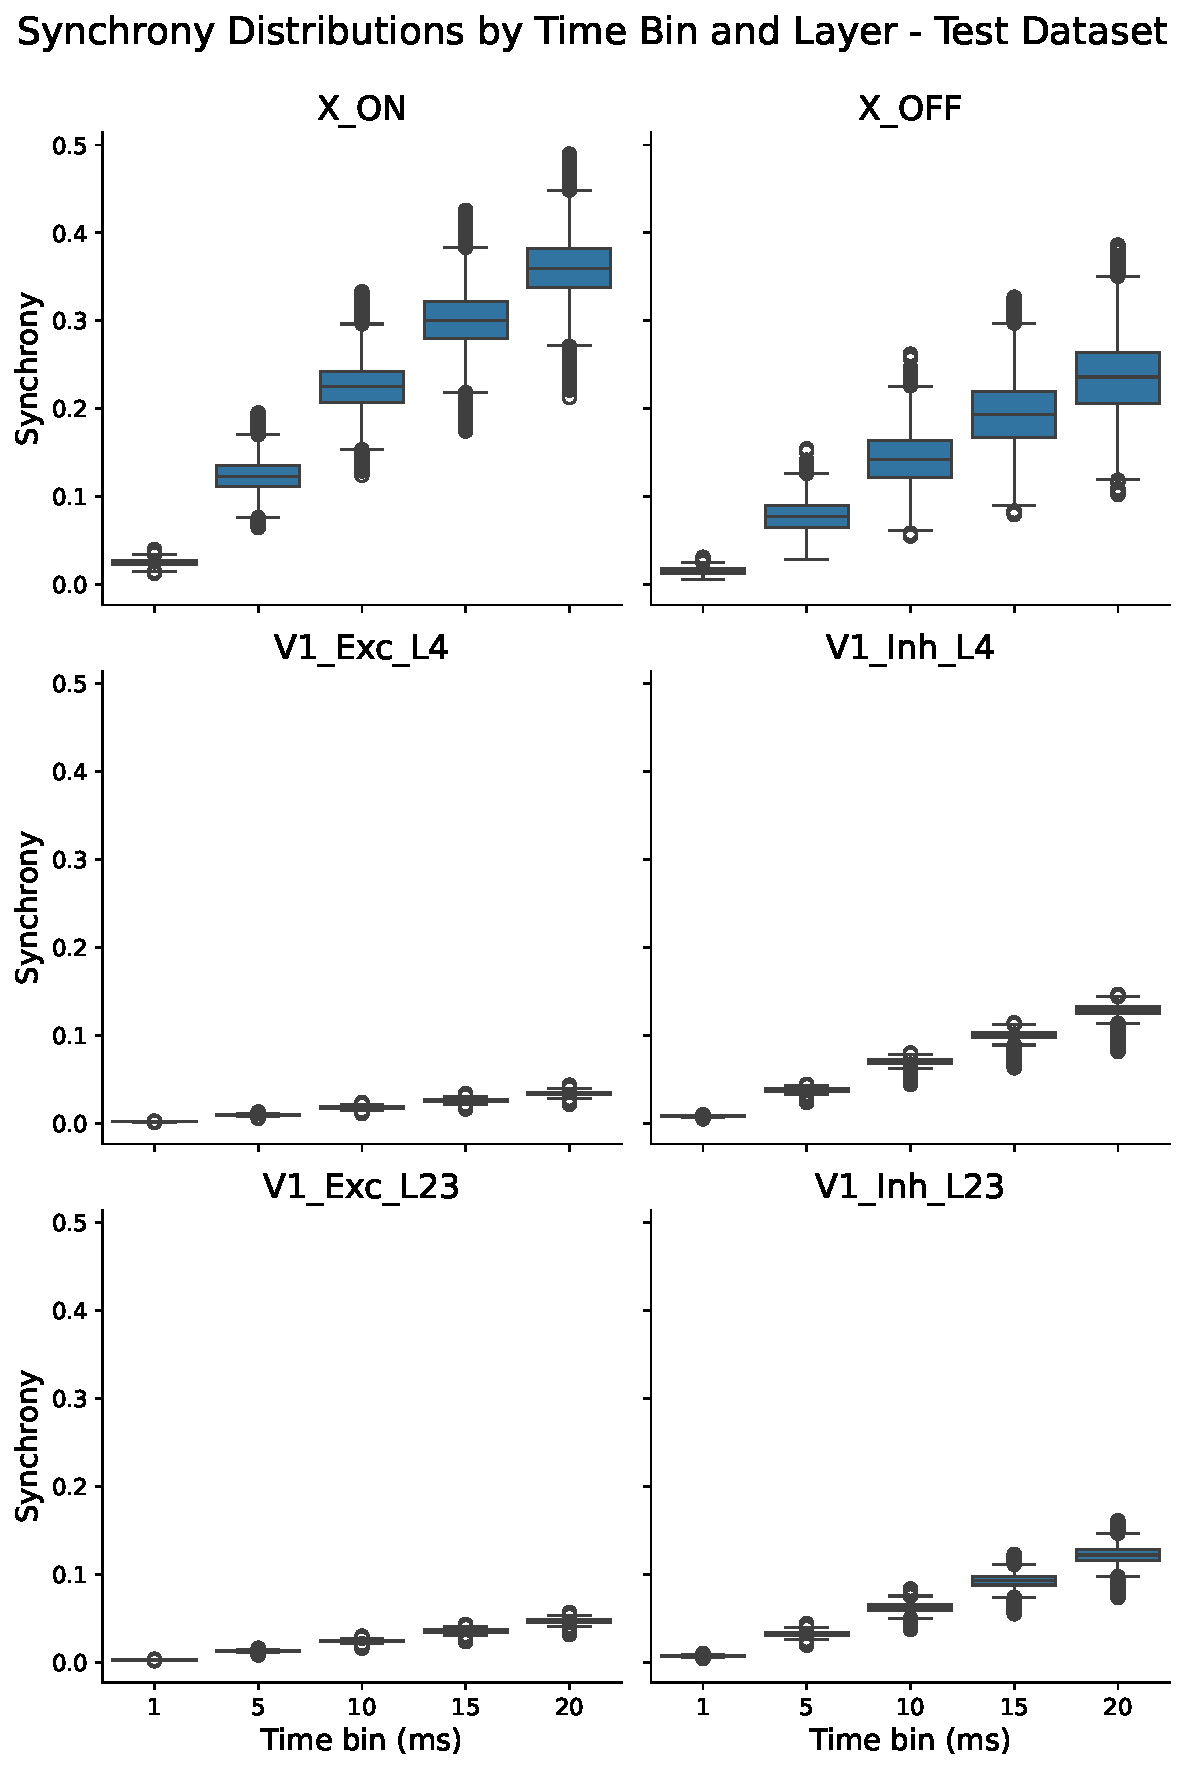
\includegraphics[width=0.92\linewidth]{img/plots/synchrony_boxplot_time_bins_test.pdf}
    \caption{Distribution of mean population synchrony across different time bin sizes for all neuronal populations in the test dataset. The boxplot represents the distribution of mean synchrony values calculated across all experiments}
    \label{fig:boxplot_synchrony_time_test}
\end{figure}

\begin{table}
    \centering\footnotesize\sf
    \begin{tabular}{lrr}
    \toprule
    time step & mean & variance \\
    \midrule
    1 & 0.0101 & 0.0001 \\
    5 & 0.0494 & 0.0018 \\
    10 & 0.0912 & 0.0057 \\
    15 & 0.1256 & 0.0098 \\
    20 & 0.1551 & 0.0134 \\
    \addlinespace % a nice non-intrusive separator of data groups (or final table sums)
    \bottomrule
    \end{tabular}
    \caption{\textbf{Summary of synchrony statistics across time bin sizes in the train dataset:} This table reports the mean and variance of population synchrony across all layers for each time bin size.}
    \label{tab:synchrony_time_bins_summary_train}
\end{table}

\begin{table}
    \centering\footnotesize\sf
    \begin{tabular}{lrr}
    \toprule
    time step & mean & variance \\
    \midrule
    1 & 0.0101 & 0.0001 \\
    5 & 0.0491 & 0.0017 \\
    10 & 0.0908 & 0.0057 \\
    15 & 0.1250 & 0.0097 \\
    20 & 0.1545 & 0.0133 \\
    \addlinespace % a nice non-intrusive separator of data groups (or final table sums)
    \bottomrule
    \end{tabular}
    \caption{\textbf{Summary of synchrony statistics across time bin sizes in the test dataset:} This table reports the mean and variance of population synchrony across all layers for each time bin size.}
    \label{tab:synchrony_time_bins_summary_test}
\end{table}

Synchrony increases with larger time bins, reflecting a higher likelihood of coincident spiking. This effect is most pronounced in LGN layers, especially X\_ON, while V1 excitatory layers show a milder change. These findings suggest that while synchrony is affected by bin size, the overall temporal dynamics are preserved.

We conclude that a bin size of 20~ms strikes a practical balance between maintaining temporal fidelity, minimizing data noise, and ensuring computational efficiency.


\subsection{Model Subset Selection Analysis}
\label{subsec:subset_selection_analysis}

In this section, we analyze the impact of selecting a subset of neurons from the original SNN model. As discussed in Section~\ref{subsubsec:subset_selection}, we selected only 10\% of the neurons due to memory constraints and the computational demands of model training. Our primary interest lies in assessing how this subset selection affects the temporal properties of the dataset, which are central to our research.

All experiments in this section are conducted on the dataset with a 20~ms time bin size (as used in our model) and focus on the training dataset unless stated otherwise. As shown previously in Section~\ref{subsubsec:time_bins_merging}, the results from the training and test datasets are largely consistent.

\subsubsection{Total Spike Counts Across Time Bins}
\label{subsubsec:total_spike_counts_subset}
We begin by analyzing the distribution of spike counts in the time bins for the full dataset and for the subset datasets. Table~\ref{tab:subset_spike_count_distribution} summarizes the mean spike count ratios across all model subsets compared to the full dataset.

\begin{table}
    \centering\footnotesize\sf
    \begin{tabular}{rrrr}
        \toprule
        Spike Count & Full Dataset Ratio & Subsets Mean Ratio & Subsets Standard Deviation \\
        \midrule
        0 & 0.9105 & 0.9102 & 0.0004 \\
        1 & 0.0710 & 0.0712 & 0.0003 \\
        2 & 0.0147 & 0.0148 & 0.0001 \\
        3 & 0.0032 & 0.0032 & 0.0000 \\
        4 & 0.0005 & 0.0005 & 0.0000 \\
        5 & 0.0001 & 0.0001 & 0.0000 \\
        \bottomrule
    \end{tabular}
    \caption{\textbf{Comparison of spike count distributions between full and subset datasets:} This table presents the mean spike count ratios and standard deviations across all model subsets, relative to the full dataset.}
    \label{tab:subset_spike_count_distribution}
\end{table}

The table shows that the differences in spike count distributions between the full and subset datasets are minimal, with low standard deviations. This suggests that randomly selecting a subset of neurons does not significantly impact the overall spike count distribution.

\subsubsection{Spike Count Distribution Across Time}
\label{subsubsec:spike_time_distribution_subset}

Next, we compare the temporal spike count distributions of the subset datasets with that of the full dataset. Figure~\ref{fig:temporal_distribution_subset_vs_full_train} shows the mean temporal behavior across layers for both the full dataset and the average of all subsets. The shaded area represents the standard deviation across subsets.
\begin{figure}
    \centering
    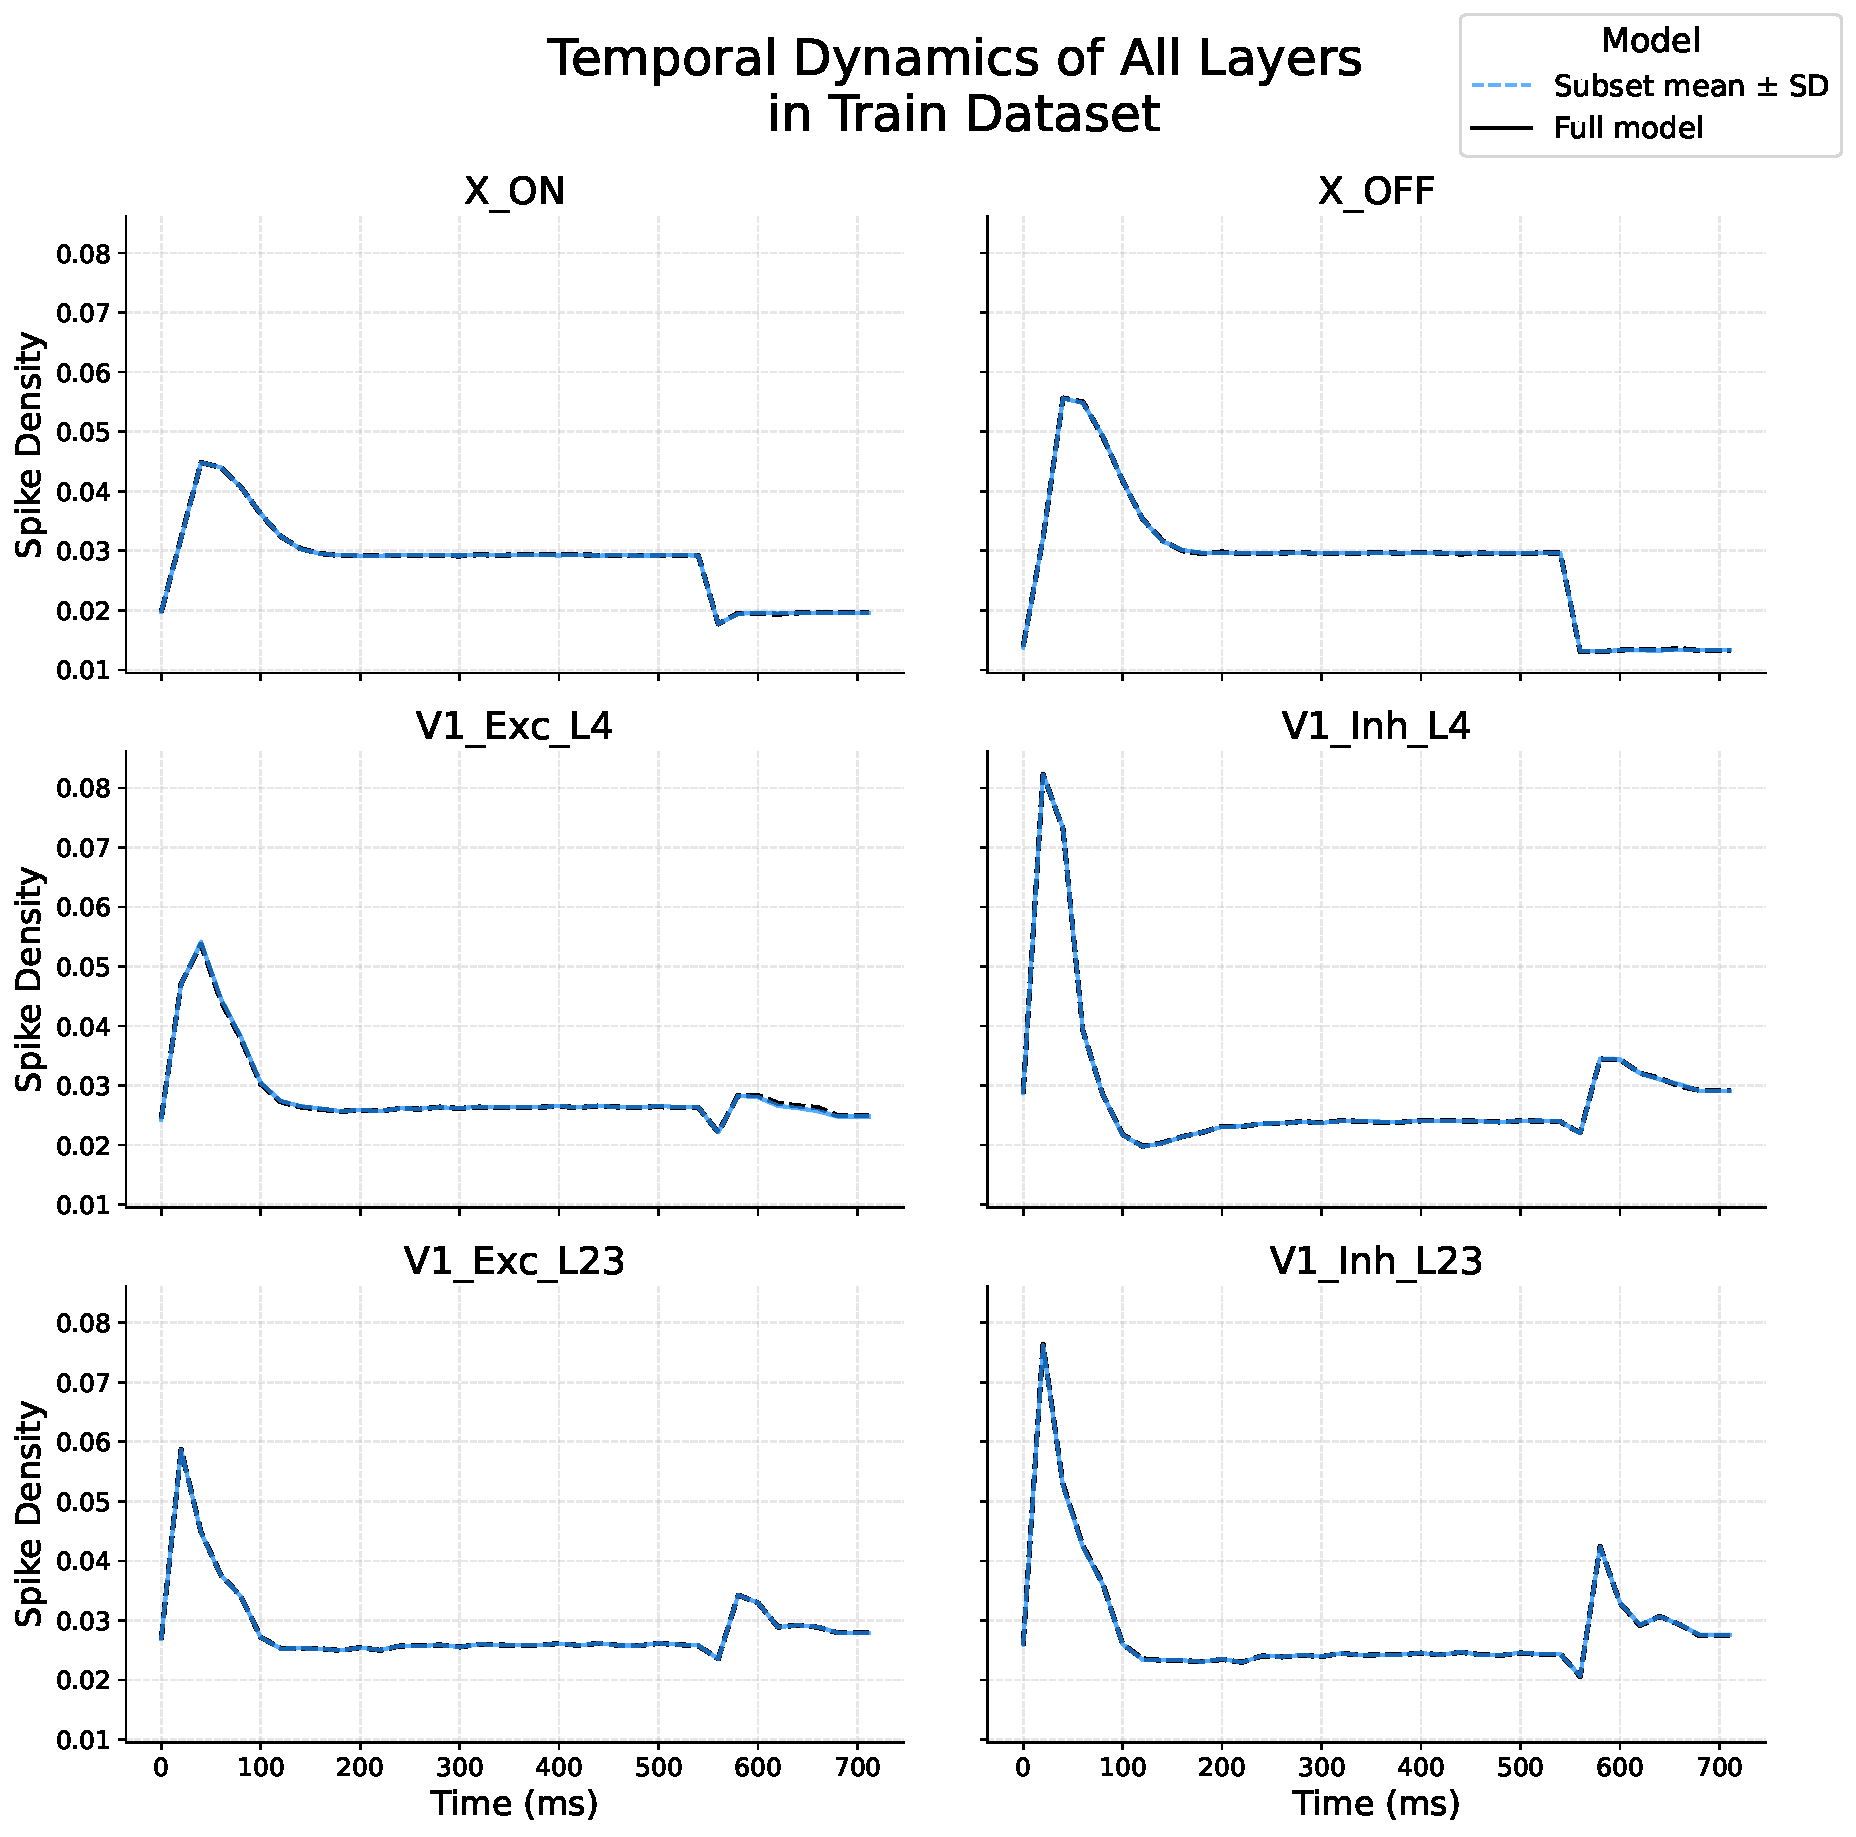
\includegraphics[width=\linewidth]{img/plots/temporal_distribution_subset_vs_full_train.pdf}
    \caption{Comparison of mean temporal activity across layers for the full dataset and the average of all subsets. The shaded area indicates the standard deviation across subsets, which is very small and therefore barely visible in the plot.}
    \label{fig:temporal_distribution_subset_vs_full_train}
\end{figure}

The plot demonstrates that the mean temporal patterns of the subsets closely match those of the full dataset. The small standard deviation further confirms that the temporal properties are preserved despite the neuron subset selection.


\subsubsection{Synchrony of Neuronal Populations in Subsets}
\label{subsubsec:neuron_synchrony_subset}
Finally, we assess the effect of subset selection on neuronal synchrony. Since we are using only a portion of the neurons from the full model, it is possible that groups of neurons that typically spike together may be disrupted, potentially affecting synchrony.

Figure~\ref{fig:boxplot_synchrony_subset} displays a boxplot and jitter plot comparing the synchrony values of the full dataset and all subsets.

\begin{figure}
    \centering
    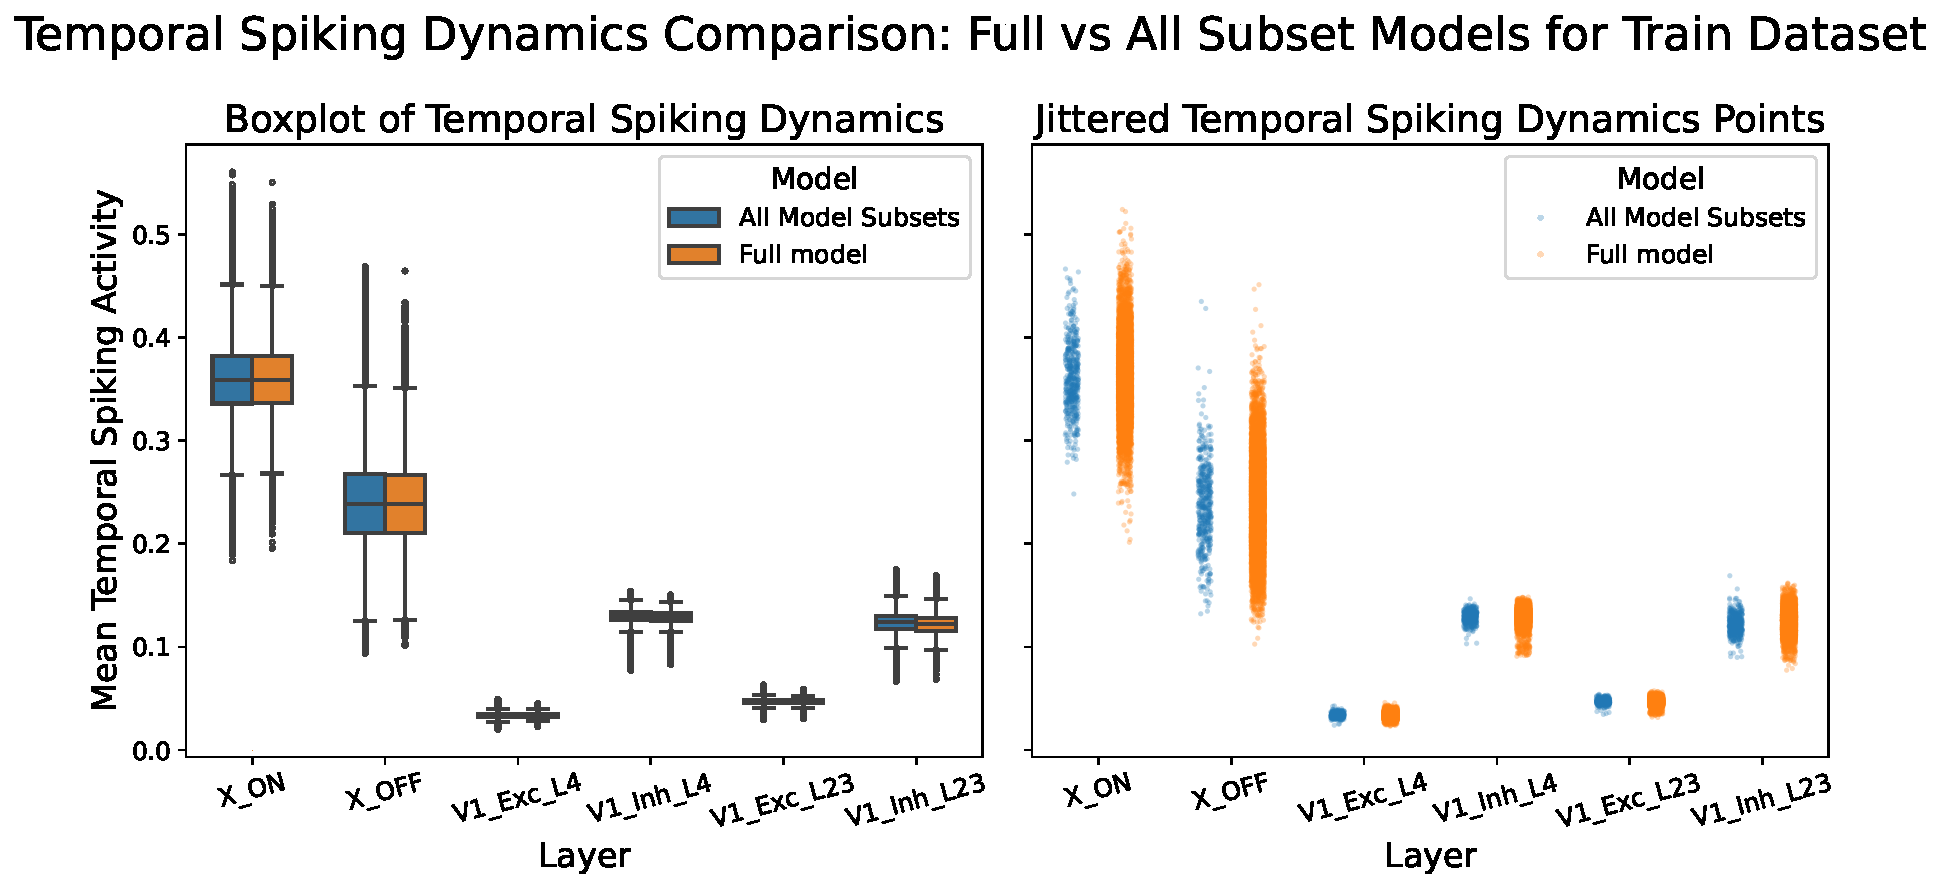
\includegraphics[width=\linewidth]{img/plots/synchrony_comparison_subset_full_train.pdf}
    \caption{Boxplot and jitter plot comparing population synchrony values between the full dataset and all subsets. Each data point represents the mean synchrony of one experiment.}
    \label{fig:boxplot_synchrony_subset}
\end{figure}

As shown, the synchrony distributions are largely similar, particularly in the excitatory layers. This aligns with earlier findings that synchrony variance was low across time bins. Although the jitter plot suggests a slightly narrower spread in the LGN layers for the subsets, the boxplots do not indicate a significant difference.

Based on these observations, we conclude that random selection of 10\% of neurons from the full SNN model does not substantially affect the dataset's statistical or temporal properties. Nevertheless, slight changes in synchrony, particularly in LGN layers, should be taken into account when interpreting model performance results.

\section{Model Evaluation}
\label{sec:model_evaluation}
